\subsection{Kalibrierung des Magnetfeldes}
Um den Zusammenhang zwischen Magnetfeldstärke und eingestelltem Strom herauszufinden, wird eine Kalibrierung-Messung durchgeführt. Dabei werden zehn Stromstärken zwischen (0-15.5)\si{\ampere} eingestellt und mit einer Hall-Sonde das zugehörige Magnetfeld gemessen. Diese Messung wird einmal mit steigenden und einmal mit fallenden Stromstärken durchgeführt, um Hysterese-Effekte zu berücksichtigen. Die gemessenen Werte sind in Abbildung \ref{fig:Hysterese} abgebildet und in Tabelle \ref{tab:Messwerte} aufgeführt. Bei den Stromstärken wird ein Ablesefehler von \SI{0.5}{\ampere} berücksichtigt. Es sind keine eindeutigen Unterschiede zwischen der Messung beim steigenden und beim fallenden Magnetfeld zu erkennen, daher wird auf einen Fit verzichtet. Statt dessen werden die Quotienten der Wertepaare zur Proportionalitätskonstante 
\begin{align}
	a = \SI{0.0572+-0.0012}{\tesla\per\ampere}

\end{align}
gemittelt.

\begin{figure}
	\centering
	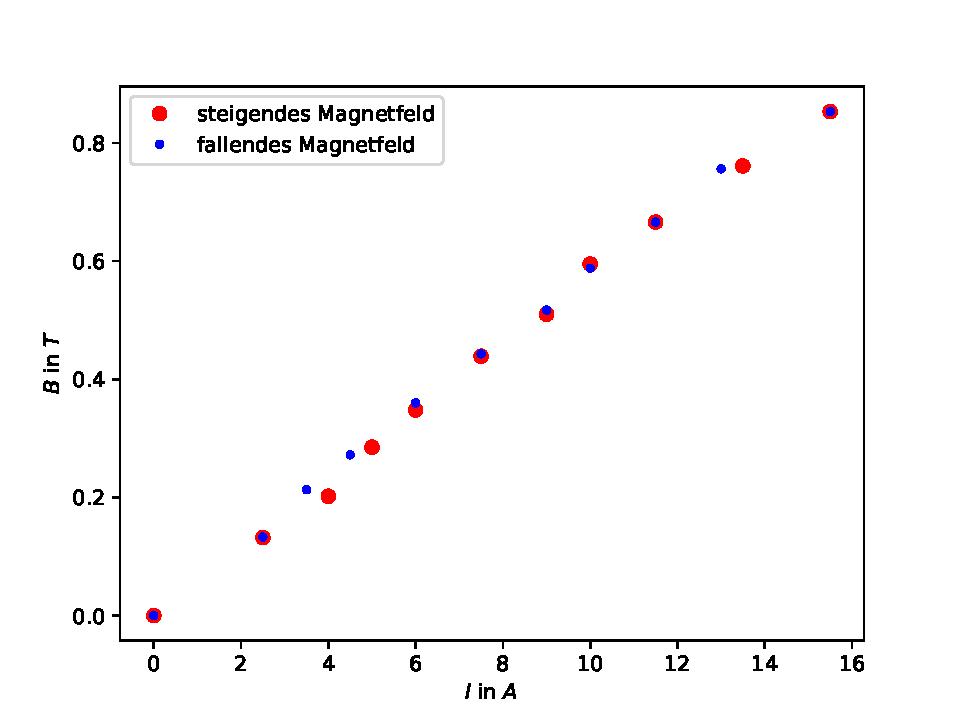
\includegraphics[width=\textwidth]{Hysterese.pdf}
	\caption{Messwerte bei der Kalibrierung des Magnetfeldes}
	\label{fig:Hysterese}
\end{figure}
\begin{table}
    \centering
    \caption{Stromstärken $I_1,I_2$ beim Auftreten des Maximums für verschiedene Anregungsfrequenzen $\nu_e$ mit dem jeweiligen Skalierungsfaktor}
    \label{tab:Werte}
    \sisetup{parse-numbers=false}
    \begin{tabular}{
	S[table-format=2.3]
	S[table-format=3.0]
	@{${}\pm{}$}
	S[table-format=2.0, table-number-alignment = left]
	S[table-format=3.0]
	@{${}\pm{}$}
	S[table-format=2.0, table-number-alignment = left]
	S[table-format=2.1]
	@{${}\pm{}$}
	S[table-format=1.1, table-number-alignment = left]
	}
	\toprule
	{$\nu_e \ \mathrm{in} \ \si{\mega\hertz}$}		& \multicolumn{2}{c}{$I_1 \ \mathrm{in} \ \si{\milli\ampere}$}		& 
	\multicolumn{2}{c}{$I_2 \ \mathrm{in} \ \si{\milli\ampere}$}		& \multicolumn{2}{c}{Skala in \si{\milli\ampere\per\centi\meter}}		\\ 
	\midrule
    10.588 & 232 & 5  & 307 & 5  & 41.5 & 0.5 \\
15.970 & 357 & 9  & 407 & 5  & 16.7 & 0.3 \\
20.560 & 453 & 9  & 546 & 4  & 18.1 & 0.3 \\
23.870 & 587 & 10 & 633 & 10 & 15.2 & 0.6 \\
29.420 & 717 & 10 & 787 & 8  & 15.3 & 0.4 \\

    \bottomrule
    \end{tabular}
    \end{table}


\subsection{Landé-Faktor}
Abbildungen \ref{fig:FotoRot} und \ref{fig:FotoBlau} zeigen die aufgenommenen Bilder für die beiden Spektrallinien. Mit einem Bildbearbeitungsprogramm wird aus den Bildern ohne Magnetfeld der Abstand zwischen den Spektrallinien gemessen. Diese Größe wird mit $\Delta s$ bezeichnet. Beim Anlegen des Magnetfelds spaltet sich jede dieser Linien in zwei Linien auf. (Bei der blauen Spektrallinie spaltet es sich eigentlich in vier Linien auf, aber das mit dieser Apparatur nicht aufgelöst werden.) Der Abstand zwischen zwei Linien, die aus derselben Linie hervorgegangen sind, wird ebenfalls ausgemessen und mit $\delta s$ bezeichnet. Die Werte für $\Delta s$ und $\delta s$ sind in den Tabellen \ref{tab:WerteFotosRot} und \ref{tab:WerteFotosBlau} zu sehen. Die Breite einer Linie ist im Bereich von 40-50 Pixeln, daher wird ein Ablesefehler von 10 Pixeln eingerechnet. Mit Hilfe von
\begin{align}
\Delta\lambda = \frac{1}{2}\frac{\delta s}{\Delta s}\Delta\lambda_\text{D}
\end{align}
kann dann die Wellenlängenverschiebung $\Delta\lambda = \lambda_0 - \lambda$ berechnet werden.

\begin{figure}[h!]
	\centering
	
\includegraphics[width=.49\textwidth]{Fotos/OhneBFeldRot.JPG} \hfill
	
\includegraphics[width=.49\textwidth]{Fotos/senkrechtRot9A.JPG}
	\caption{Aufgenommene Bilder bei der roten Spektrallinie. Links ohne Magnetfeld, rechts mit Magnetfeld und senkrechtem Polarisationsfilter.}
	\label{fig:FotoRot}
\end{figure}
\begin{figure}[h!]
	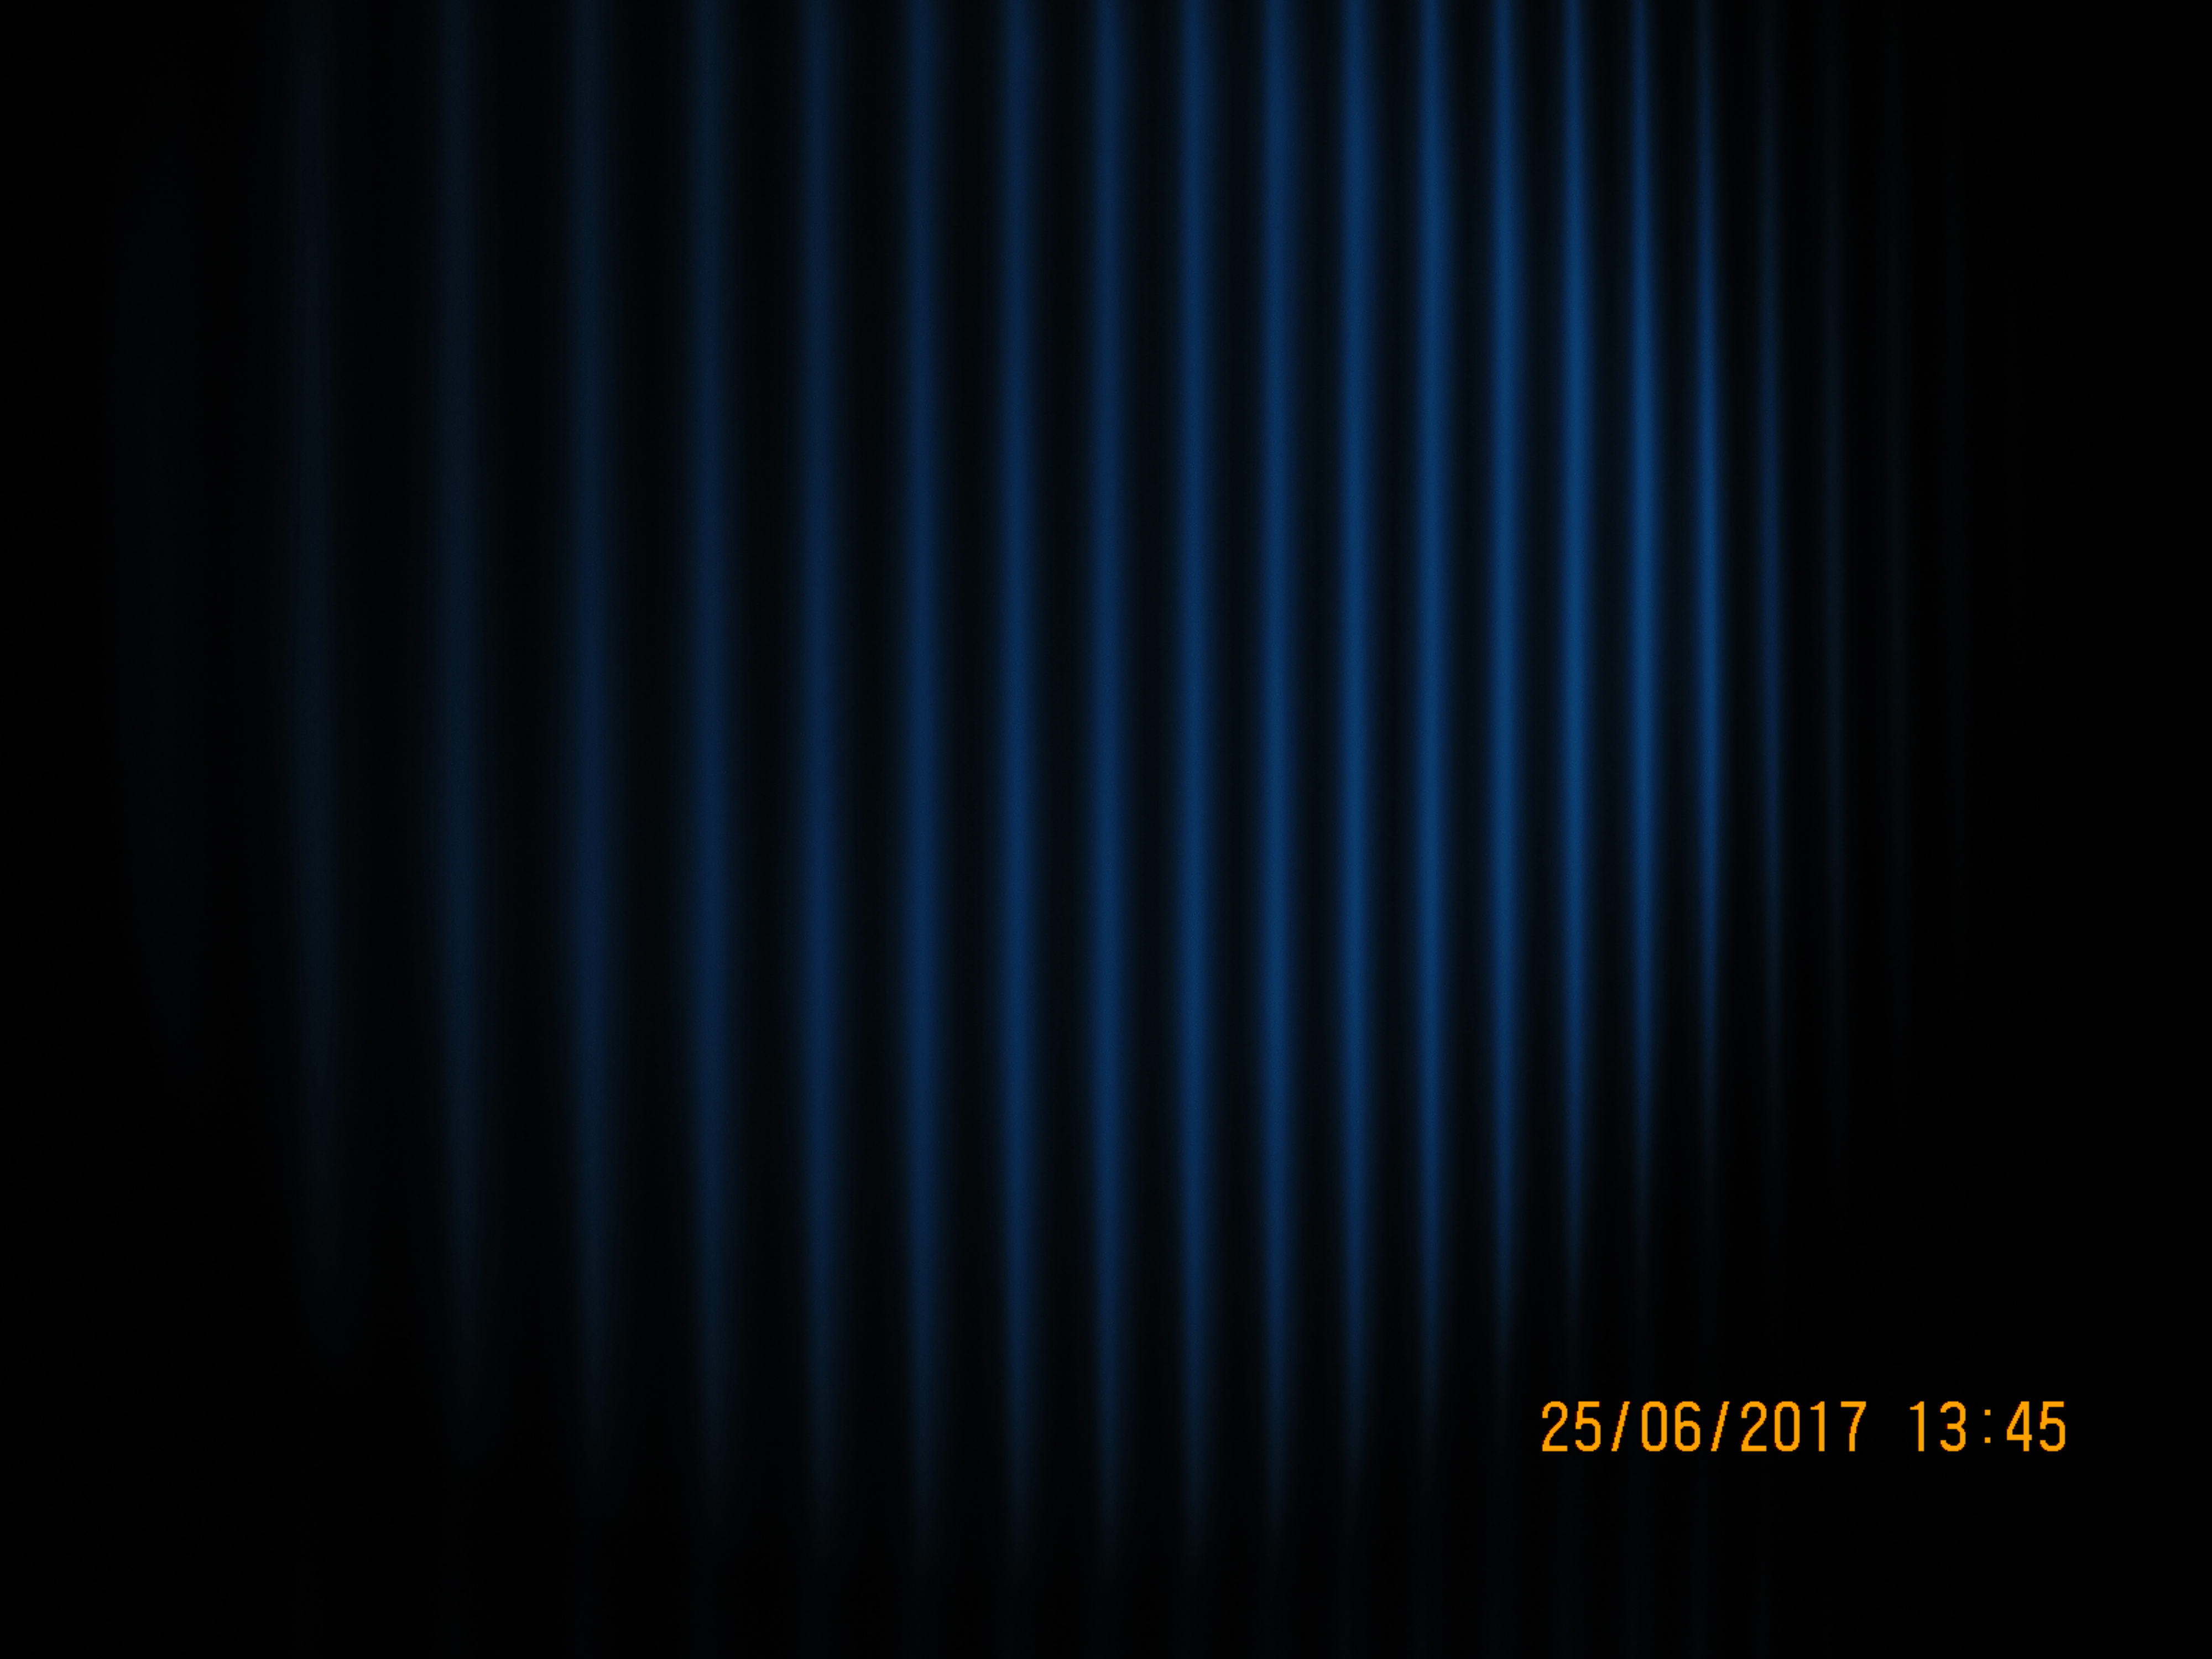
\includegraphics[width=.32\textwidth]{Fotos/OhneBFeldBlau.JPG} \hfill
	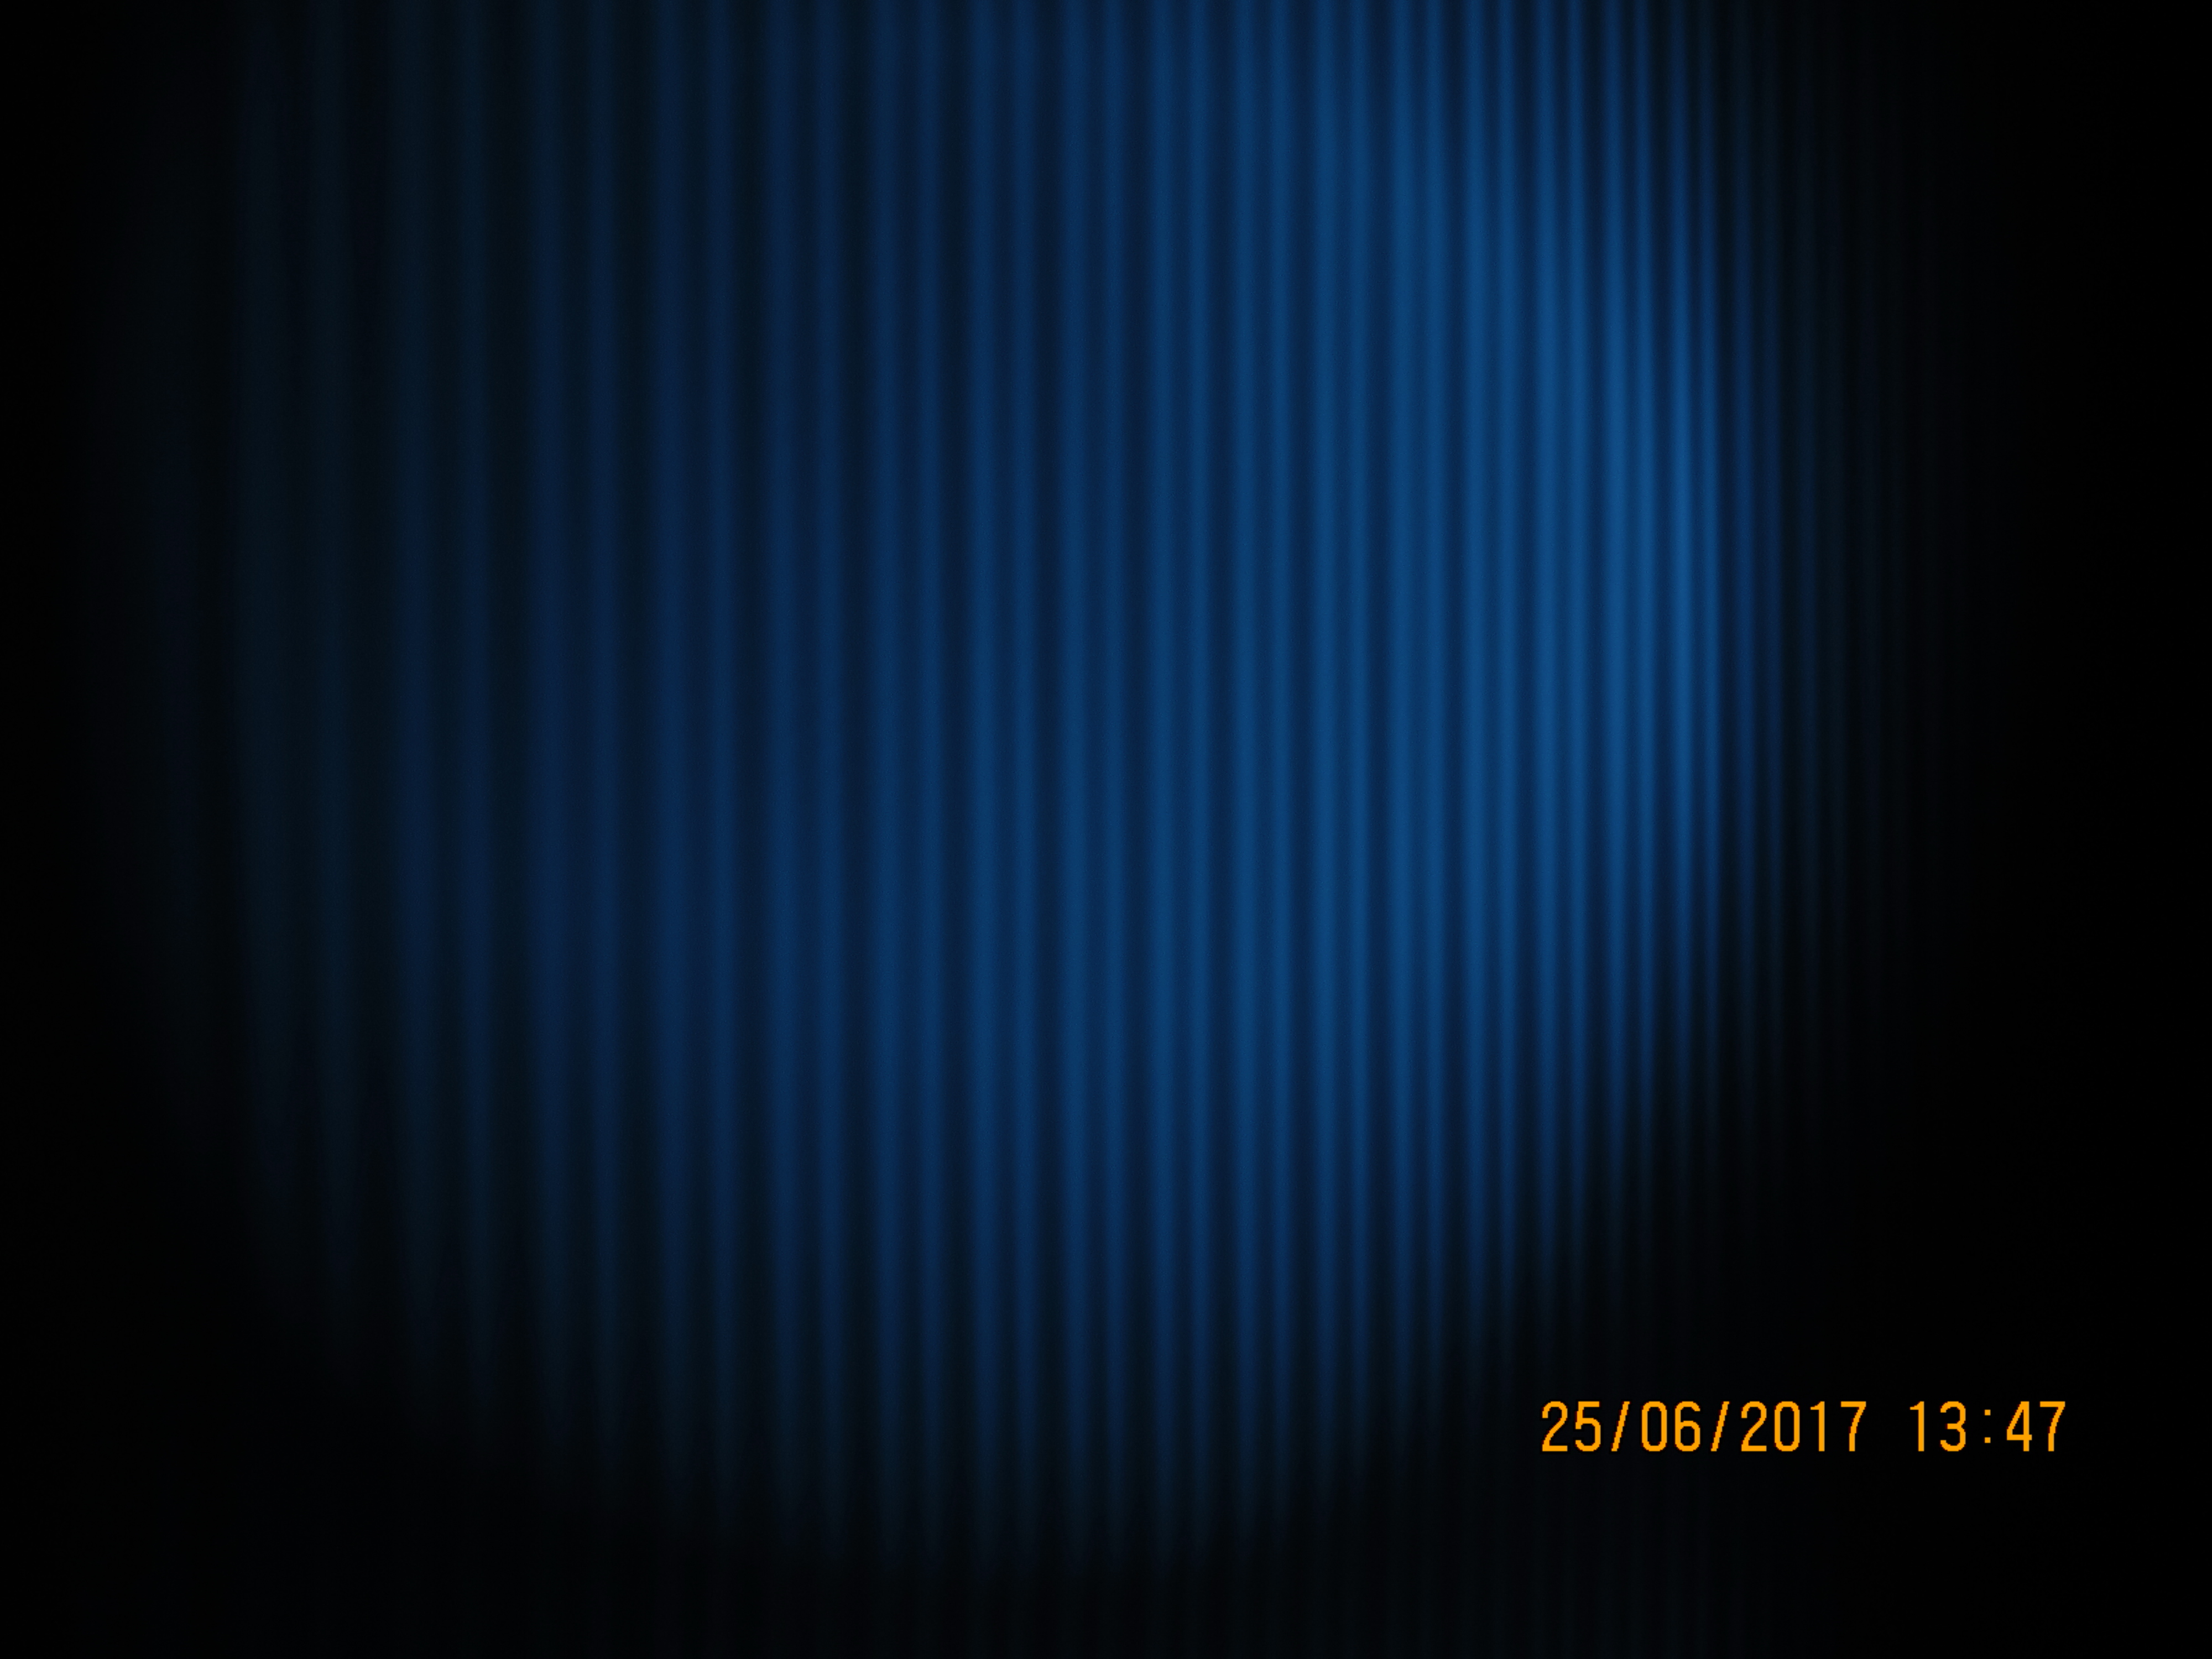
\includegraphics[width=.32\textwidth]{Fotos/senkrechtBlau5A.JPG} \hfill
	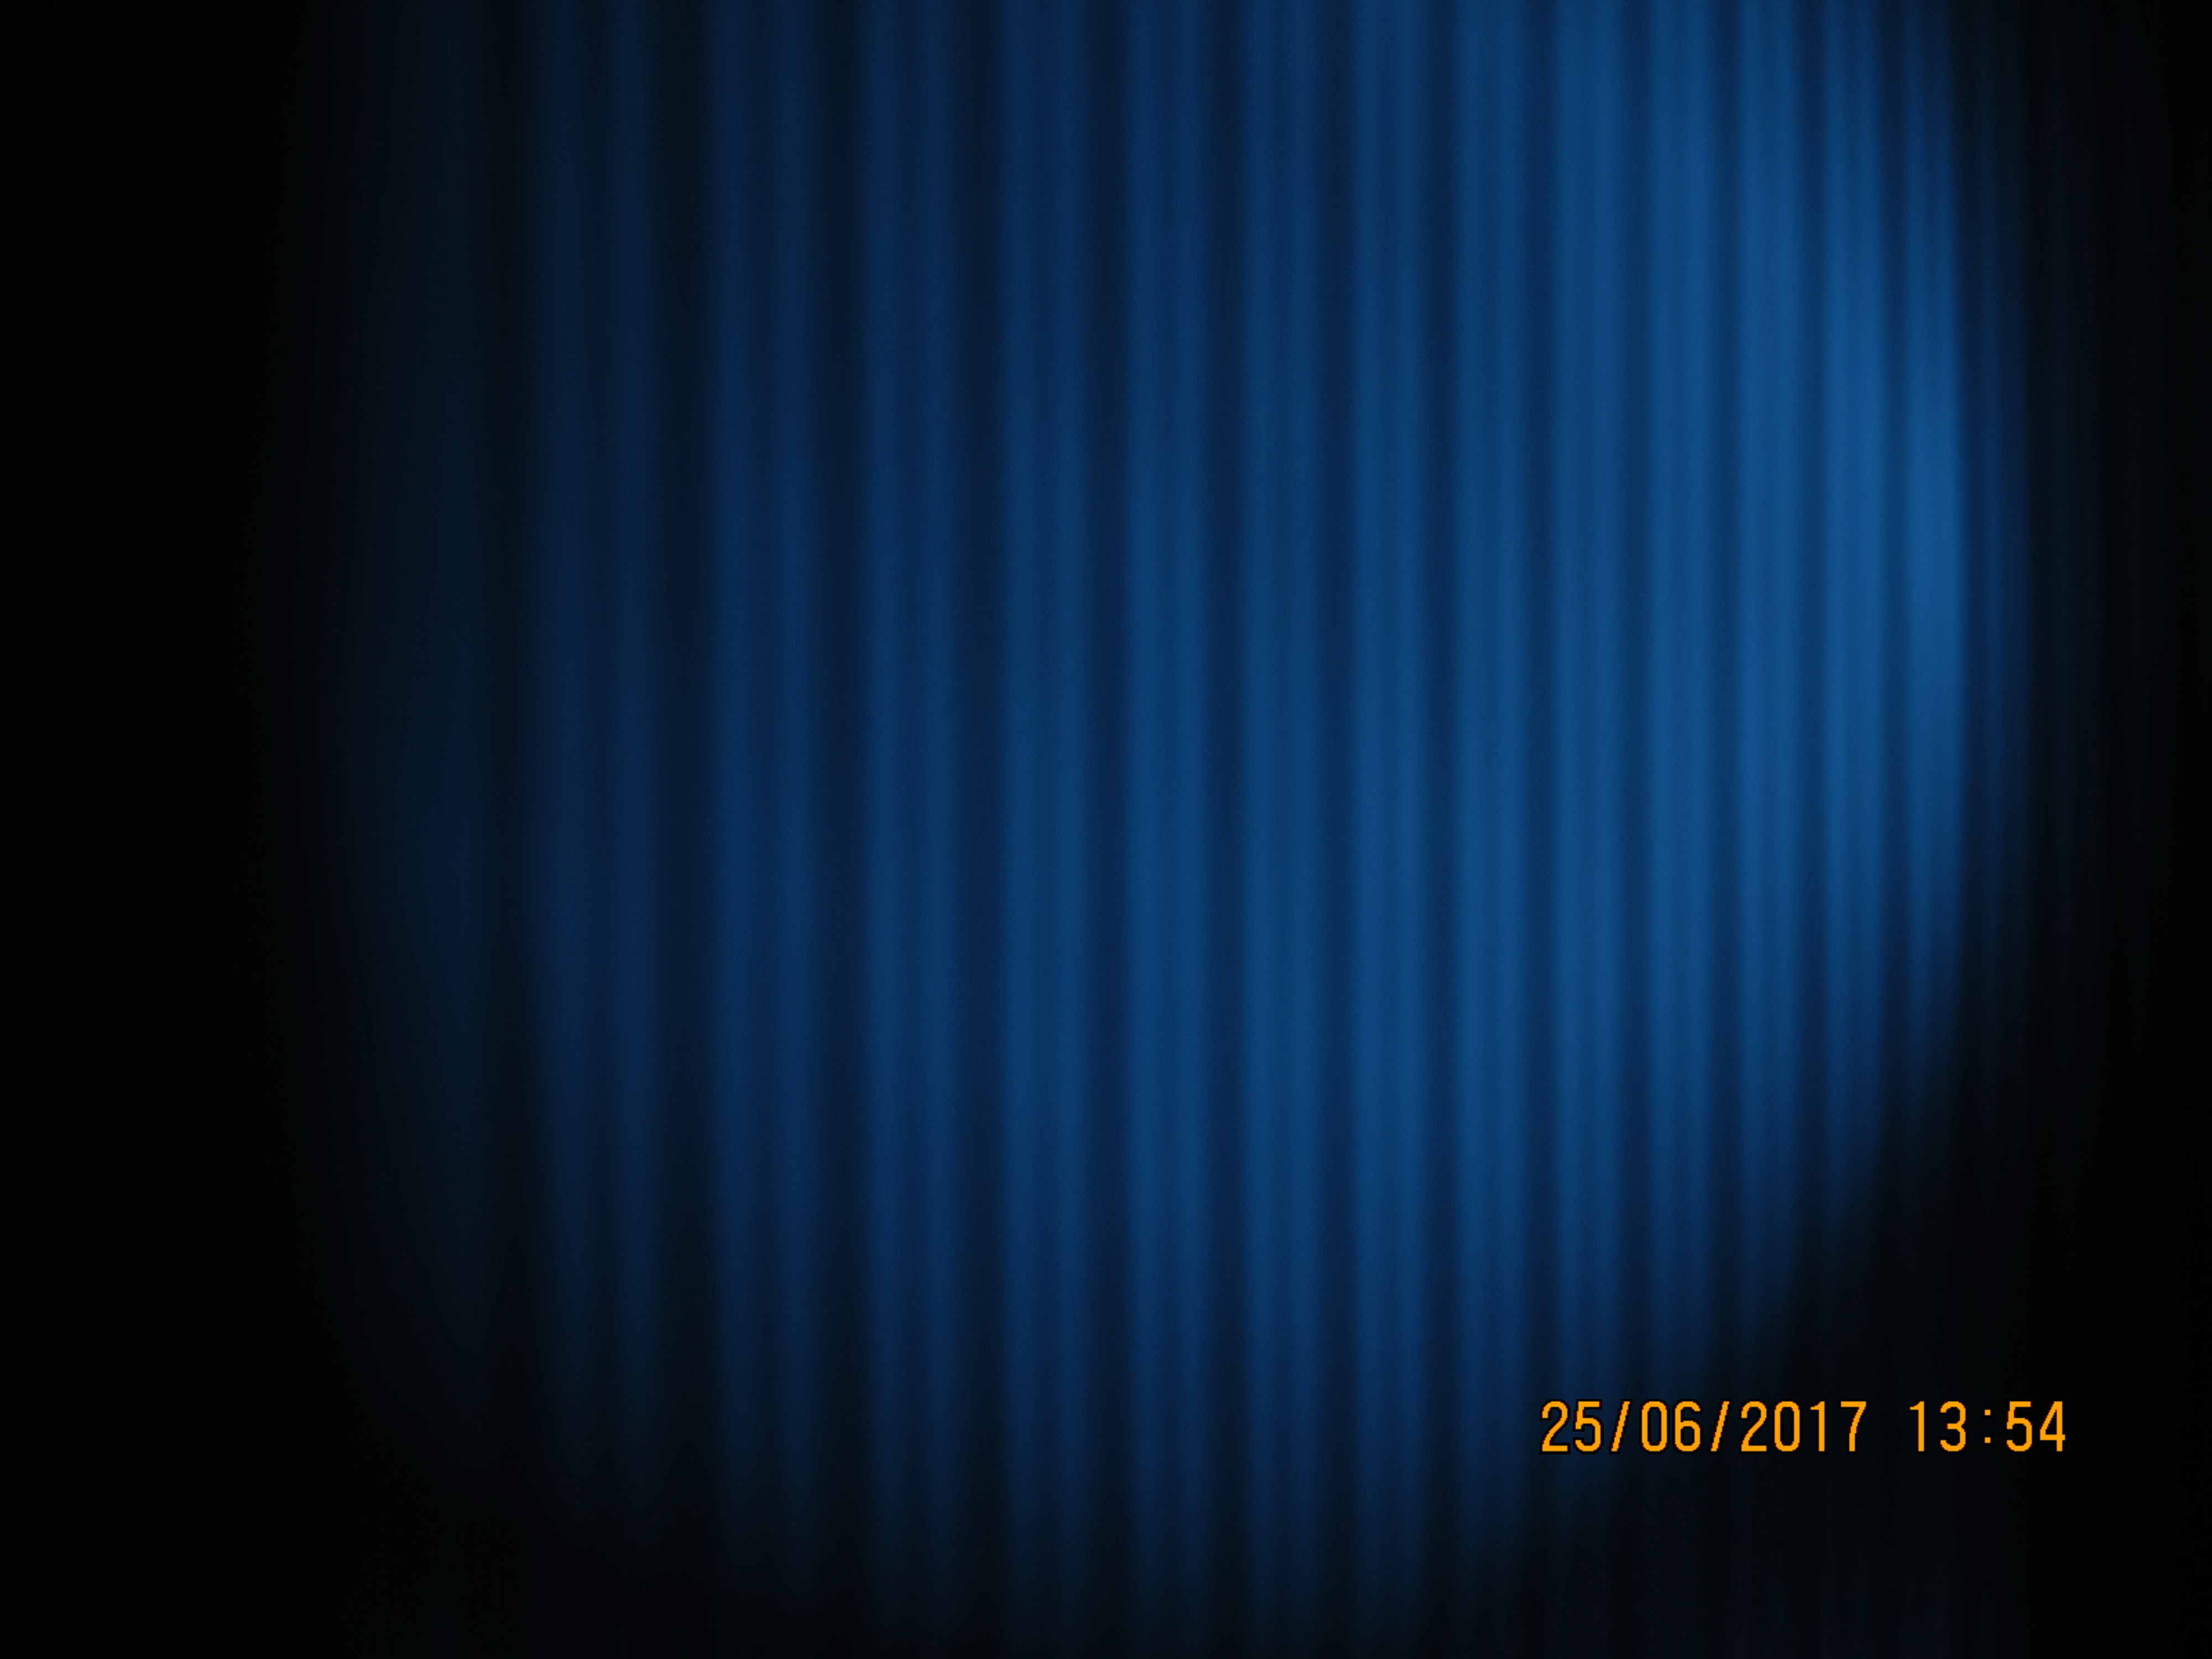
\includegraphics[width=.32\textwidth]{Fotos/parallelBlau15A.JPG}
	\caption{Aufgenommene Bilder bei der blauen Spektrallinie. Links ohne Magnetfeld, mittig mit Magnetfeld und senkrechtem Polarisationsfilter, rechts mit Magnetfeld und parallelem Polarisationsfilter.}
	\label{fig:FotoBlau}
\end{figure}\ \\ \ \\

Die Änderung der Energiedifferenz zwischen zwei Niveaus beim Einschalten eines Magnetfeldes, $dE$, kann durch die Wellenlänge eines beim Übergang emittierten Photons ausgedrückt werden:
\begin{align*}
	dE &= E(B\not=0) - E(B=0) = \frac{hc}{\lambda} - \frac{hc}{\lambda_0} \ .
\end{align*}
Der erste Term wird durch die ersten beiden Glieder seiner Taylor-Reihe ausgedrückt
\begin{align*}
	\frac{hc}{\lambda}\approx\frac{hc}{\lambda_0}-\frac{hc}{\lambda_0^2}(\lambda-\lambda_0) \ .
\end{align*}
Für die Änderung der Energiedifferenz gilt dann
\begin{align}
	dE = \frac{hc}{\lambda_0^2}\Delta\lambda \ .
\end{align}
Durch Gleichsetzen mit \eqref{eq:Energieverschiebung} kann so der Landé-Faktor
\begin{align}\label{eq:Lande}
	g_{12} = \frac{dE}{\mu_\text{B}B} = \frac{hc}{\mu_\text{B}B}\frac{\Delta\lambda}{\lambda_0^2}
\end{align}
berechnet werden. Neben den physikalischen Konstanten $h,c,\mu_\text{B}$, werden die Magnetfeldstärke $B$ und die Wellenlänge $\lambda_0$ benötigt:
\begin{align*}
	B_{\text{red,}\sigma}= &\SI{514(11)}{\milli\tesla} \quad && \quad &\lambda_{\text{red},0} = &\SI{643.8}{\nano\meter} \\
	B_{\text{blue,}\sigma}= &\SI{286(6)}{\milli\tesla} \quad && \quad &\lambda_{\text{blue},0} = &\SI{480.0}{\nano\meter} \\
	B_{\text{blue,}\pi}= &\SI{857(18)}{\milli\tesla} \ . && & & &
\end{align*}
Gemittelt ergeben sich so die Landé-Faktoren
\begin{align}
	g_{\text{red,}\sigma} &= \SI{1.12+-0.08}{}
\notag \\
	g_{\text{blue,}\sigma} &= \SI{2.1+-0.2}{}
\notag \\
	g_{\text{blue,}\pi} &= \SI{0.57+-0.06}{}
 \ .
\end{align}

\begin{table}
    \centering
    \caption{Abstände $\Delta s,\delta s$ in Pixel bei der roten Linie}
    \label{tab:WerteFotosRot}
    \sisetup{parse-numbers=false}
    \begin{tabular}{
	S[table-format=3.0]
	S[table-format=3.0]
	}
	\toprule
	{$\Delta s_\mathrm{red}$}		& {$\delta s_{\mathrm{red,}\sigma}$}		\\ 
	\midrule
    266 & 114 \\
250 & 112 \\
238 & 108 \\
216 & 96  \\
206 & 96  \\
196 & 94  \\
188 & 84  \\
180 & 84  \\
178 & 82  \\
168 & 76  \\
162 & 74  \\
160 & 72  \\
156 & 72  \\
148 & 66  \\
148 & 66  \\
140 & 64  \\

    \bottomrule
    \end{tabular}
    \end{table}

\begin{table}
    \centering
    \caption{Abstände $\Delta s,\delta s$ in Pixel bei der blauen Linie}
    \label{tab:WerteFotosBlau}
    \sisetup{parse-numbers=false}
    \begin{tabular}{
	S[table-format=3.0]
	S[table-format=3.0]
	S[table-format=2.0]
	}
	\toprule
	{$\Delta s_\mathrm{blue}$}		& {$\delta s_{\mathrm{blue,}\sigma}$}		& 
	{$\delta s_{\mathrm{blue,}\pi}$}		\\ 
	\midrule
    224 & 108 & 96 \\
196 & 96  & 85 \\
188 & 88  & 78 \\
176 & 84  & 73 \\
164 & 80  & 65 \\
156 & 72  & 62 \\
152 & 72  & 61 \\
144 & 68  & 61 \\
148 & 64  & 55 \\
132 & 64  & 49 \\
132 & 60  & 47 \\
128 & 60  & 50 \\
124 & 56  & 41 \\
108 & 52  & 35 \\

    \bottomrule
    \end{tabular}
    \end{table}

